% ============================================================================
% The Spike-Reset Boundary -- IEEE conference submission (LaTeX port).
% Ported from paper/continuous_lens.typ. Double-blind / anonymized byline.
%
% BUILD:
%   pdflatex main && bibtex main && pdflatex main && pdflatex main
% ============================================================================
\documentclass[conference]{IEEEtran}
\IEEEoverridecommandlockouts

\usepackage{cite}
\usepackage{amsmath,amssymb,amsfonts}
\usepackage{graphicx}
\usepackage{textcomp}
\usepackage{xcolor}
\usepackage[hidelinks]{hyperref}
\renewcommand{\ttdefault}{cmtt} % Courier (pcr) TFM unavailable in this TeX install

\begin{document}

\title{The Spike-Reset Boundary: When Continuous Analysis of\\
Spiking-Network Archetypes Holds, and When It Does Not}

\author{\IEEEauthorblockN{Anonymous Author(s)}
\IEEEauthorblockA{Affiliation withheld for double-blind review}}

\maketitle

\begin{abstract}
Formal verification of spiking neural networks (SNNs) encodes small leaky
integrate-and-fire (LI\&F) network \emph{archetypes} as discrete transition
systems and discharges temporal-logic properties to a model checker. This is
exact but exponential, and it certifies a property at a parameter point without
describing the \emph{shape} of the region where the property holds. We ask
whether the classical, continuous machinery of dynamical systems ---
eigenvalues, transfer functions, bifurcation theory --- can supply that shape.
We answer with a complete two-sided account. On one side, continuous methods
recover shape and scale precisely: a single eigenvalue predicts the
winner-take-all boundary at 99.96\% in a mean-field description; the
winner-take-all and oscillation-onset boundaries are exact closed-form curves;
a diffusion-approximation firing-rate formula yields a 99.6\%-recall envelope
of the verified winner-take-all region, usable as a sound model-checking
pre-filter. On the other side, every continuous method systematically misses
the integer-tick spike-timing physics --- the exact staircase of
synchronous-lock cells, the exact oscillation period, the binary spike
waveform. We identify the single mechanism responsible: the \emph{spike-reset
rule}. We show that whether the reset is load-bearing for a given property is a
\emph{decidable, a-priori test} for whether continuous analysis is sound for
it, and we confirm the test through both its positive and its negative
predictions. The methods form a fidelity/tractability \emph{ladder} from
linearization to discrete model checking; we close with a multi-scale workflow
that places a sound polynomial-cost continuous pre-filter in front of an
exponential model checker. Negative results are reported as primary evidence:
they measure precisely how much of a verified property is irreducibly discrete.
\end{abstract}

\begin{IEEEkeywords}
spiking neural networks, formal verification, leaky integrate-and-fire,
mean-field analysis, bifurcation theory, model checking
\end{IEEEkeywords}

% ============================================================================
\section{Introduction}\label{sec:intro}
% ============================================================================

Spiking neural networks (SNNs) \cite{maass1997networks} model computation with
discrete, all-or-nothing spikes. Small SNN motifs --- two neurons inhibiting
each other, an activator--inhibitor feedback loop --- recur as functional
primitives, and a line of work initiated by De Maria et al.
\cite{DeMaria2020,naco20}, which we abbreviate \emph{FCS}, established these
\emph{archetypes} as targets for \emph{formal verification}: each archetype is
encoded as a discrete transition system and its behavioural properties (a
winner emerges; the network oscillates) are discharged to a model checker. The
CogSpike programme \cite{cogspike_wd} extends this with a probabilistic neuron
model, a Markov-chain encoding, and PRISM-based \cite{PRISM2011} verification,
together with a weight-discretization abstraction that fights the
\emph{state-space explosion problem} --- the transition system grows
exponentially with neuron count.

Discrete verification of this kind is \emph{sound and exact}, and it is the
right tool for a yes/no question about a specific design. But it has two
structural limitations. It is \emph{exponential} in network size. And it
verifies a property \emph{at a point}: one integer weight assignment at a time.
It does not return the \emph{shape} of the region of parameters where a
property holds, the \emph{margin} before the property breaks, or \emph{why} it
holds. A designer sweeping a parameter grid re-runs an exponential procedure at
every cell.

The mathematics of \emph{dynamical systems} --- differential equations,
eigenvalues, transfer functions, bifurcation theory --- was built to answer
exactly the questions a model checker does not: where a behaviour's boundary
lies in parameter space, how fast a system settles, what happens just past the
boundary. It is, however, the mathematics of \emph{continuous, smooth} systems,
and a spiking neuron is neither: when it fires, its state \emph{resets}
discontinuously. This paper asks whether the continuous toolkit can nonetheless
be brought to bear on LI\&F archetypes, and --- crucially --- delimits exactly
when it can.

\textbf{Contributions.} (i) We give a continuous analysis suite for LI\&F
archetypes spanning static, dynamic, and finite-size regimes, and validate it
against a bit-exact discrete oracle. (ii) We characterise winner-take-all as
\emph{two distinct mathematical objects} depending on the verification
semantics --- combinatorial under deterministic semantics, spectral under
reachability semantics --- and give a sound spectral certificate for the
latter. (iii) We state and confirm a \emph{diagnostic principle}: the
spike-reset rule is the nonlinearity continuous analysis erases, and its
presence in a property is a decidable test for whether continuous methods are
sound for it. (iv) We report the \emph{negative results} --- four failed
hypotheses --- as primary evidence, since each falls exactly where the
principle predicts and together they \emph{measure} the boundary of continuous
analysis. (v) We organise the methods into a fidelity ladder and a multi-scale
verification workflow.

This paper is the continuous companion to the discrete CogSpike paper
\cite{cogspike_wd}: same archetypes, same winner-take-all case study, opposite
lens. Where that paper makes exact verification cheaper by shrinking the
transition system, this paper asks where continuous approximation can replace
exact verification entirely --- and proves where it cannot. A comprehensive
internal report develops every thread in full \cite{synthesis}; this paper
distils the publishable narrative.

% ============================================================================
\section{Background}\label{sec:background}
% ============================================================================

This section is deliberately generous. The continuous toolkit is standard in
dynamical-systems theory but not in formal verification; we introduce each
concept from first principles, assuming no background in differential equations
or control theory.

\subsection{The FCS LI\&F neuron and two archetypes}\label{sec:fcs}

A \emph{leaky integrate-and-fire} (LI\&F) neuron integrates weighted input into
a membrane potential, leaks a fraction of it away each step, and emits a spike
--- then resets --- when the potential crosses a threshold. The FCS neuron
\cite{DeMaria2020} is a discrete-time instance: it keeps a length-$5$ memory of
recent weighted inputs, combines them with fixed coefficients $[10,5,3,2,1]$
into a potential $V(t)$, fires when $V(t) \geq 105$, exports the spike one tick
later, and --- the feature this paper turns on --- \emph{zeroes the shifted
memory taps on the tick after a spike}. That zeroing is the \emph{reset}. A
neuron driven by constant input of weight $\geq 11$ fires immediately and is
called a \emph{delayer}.

Two archetypes recur throughout. \emph{Contralateral inhibition}: two neurons,
each externally driven, each inhibiting the other; its behaviour of interest is
\emph{winner-take-all} (WTA) --- one neuron fires steadily, the other falls
silent. \emph{The negative loop}: an activator $A$ excites an inhibitor $I$,
which inhibits $A$ back; its behaviour of interest is \emph{oscillation} ---
under constant drive, $A$ settles into a periodic spike pattern. FCS verifies
WTA as its Property 7 and the period-$4$ oscillation pattern \texttt{1100} as
its Property 5.

\subsection{The continuous toolkit: a ladder of six methods}\label{sec:toolkit}

A spiking network is a \emph{dynamical system}: a state (the membrane
potentials) advanced by a rule. The rule's subthreshold part --- integrate and
leak --- is \emph{linear} and completely understood; its spiking part ---
threshold and reset --- is nonlinear and \emph{discontinuous}. The six analysis
methods used in this paper differ only in how they handle that discontinuity.
They form a \emph{ladder}, from coarsest and cheapest to most faithful and most
expensive.

\textbf{Rung 1 --- linearization and eigenvalues.} A linear rule $x \to M x$ is
solved by the \emph{eigenvalues} of $M$: numbers $\lambda$ such that some
direction is simply rescaled by $\lambda$ each step. $|\lambda| < 1$ means that
direction decays; $|\lambda| > 1$ means it grows. The \emph{spectral radius}
$\rho(M) = \max|\lambda|$ is the one number deciding whether the system
settles. Linearizing the network's dynamics near an operating point and taking
$\rho$ is rung 1. A formal-methods reader knows this test in another guise:
$\rho < 1$ is the convergence condition of a fixed-point iteration, and the gap
between the top eigenvalue and the rest is the analogue of a Markov chain's
spectral gap. Cost: $O(n^3)$, negligible.

\textbf{Rung 2 --- transfer functions.} Eigenvalues describe relaxation in
isolation; a \emph{transfer function} $H(\omega)$ describes the response to a
driving input that oscillates at frequency $\omega$. A linear system responds
at the same frequency, rescaled and phase-delayed; $H(\omega)$ records both.
The one fact to keep: a leaky neuron is a \emph{low-pass filter} --- it follows
slow input and ignores fast input. Plotting $|H(\omega)|$ is a Bode plot; it
reads off ringing frequencies and stability margins.

\textbf{Rung 3 --- mean-field (Wilson--Cowan).} Rungs 1--2 silently replaced the
hard threshold with a smooth curve. Rung 3 derives that curve. Replace one
neuron by a \emph{population} of many similar neurons with slightly spread
thresholds, and track the \emph{fraction} firing. Because thresholds are
spread, the fraction is a \emph{smooth} function of input --- the single-neuron
reset is averaged away by the crowd. The population rate obeys a smooth
differential equation, the \emph{Wilson--Cowan equation} \cite{WilsonCowan1972},
and smooth equations are what \emph{bifurcation theory} needs: the analytic
boundaries of behaviour are the parameter values where a fixed point changes
stability.

\textbf{Rung 4 --- the Siegert closed form.} Rung 3 still needs a gain curve,
hand-tuned so far. Siegert's $1951$ formula \cite{Siegert1951,Brunel2000}
derives it from the neuron's own physics: a neuron integrating noisy input has
a firing rate given in closed form by the input's mean and variance. No fitting
knobs --- every quantity is a measurable property of the neuron.

\textbf{Rung 5 --- quasi-renewal mesoscopics.} Mean-field theory is exact only
for infinitely many neurons. A finite population is \emph{noisy} (fluctuations
scale as $1/\sqrt{N}$) and has \emph{age structure} (time since each neuron last
fired). The quasi-renewal equations \cite{NaudGerstner2012} track both.
Tracking age is how the reset re-enters the description: a neuron that just
fired is ``young'' and cannot fire again at once. Rung 5 is the first rung that
carries the reset.

\textbf{Rung 6 --- the discrete oracle.} The bottom rung is the FCS neuron
itself, simulated or model-checked exactly --- every tick, every reset. It
answers everything, bit-exactly, at exponential cost. It is the reference
against which rungs 1--5 are measured, and its cost is the reason rungs 1--5
exist.

\begin{table*}[t]
\caption{The methodology ladder. Each rung restores one more piece of the spike
physics the rung above discarded; the boundary between rungs 1--5 and rung 6 is
the spike-reset rule.}
\label{tbl:ladder}
\centering
\begin{tabular}{|c|l|l|l|}
\hline
\textbf{Rung} & \textbf{Method} & \textbf{What it computes} & \textbf{Cost} \\
\hline
1 & Linearization / $\rho(A)$ & stability, convergence, reachability & $O(n^3)$ \\
\hline
2 & Transfer function $H(\omega)$ & frequency response, ringing, margins & $O(n^3)$ \\
\hline
3 & Wilson--Cowan mean-field & bifurcation \emph{curves} --- behaviour boundaries & $O(n^3)$+sym. \\
\hline
4 & Siegert closed form & physical fixed points; the WTA \emph{envelope} & calib.+roots \\
\hline
5 & Quasi-renewal mesoscopics & finite-size effects; oscillation \emph{period} & stoch. sim. \\
\hline
6 & Discrete FCS oracle & everything, bit-exact & exponential \\
\hline
\end{tabular}
\end{table*}

\subsection{The discrete oracle and a caveat}\label{sec:oracle}

Throughout, ``the FCS oracle'' is a re-implementation of the FCS LI\&F
semantics run forward tick by tick, used as ground truth. The original FCS
Lustre source was not available to us; all comparisons are to this
re-implementation of the published semantics. The continuous methods were
developed and validated against the \emph{deterministic} FCS LI\&F neuron; the
probabilistic neuron of the companion CogSpike paper \cite{cogspike_wd} is a
separate variant of the same model.

% ============================================================================
\section{Two regimes of winner-take-all}\label{sec:wta}
% ============================================================================

Our lead case study is contralateral-inhibition winner-take-all: FCS Property
7, plotted in FCS's Figure 10 over a $40 \times 40$ grid of the two inhibitory
weights. Reproducing the discrete oracle gives 63.4\% WTA-stable cells. The
striking structure is \emph{three diagonal blocks of red} --- bands of weights
where, instead of a winner, the two neurons fall into a \emph{synchronous
lock}, firing in identical lockstep (at period $2$, $3$, or $4$ across weak,
medium, and strong weights). We call this the \emph{staircase}; it is the
recurring antagonist of the paper.

\subsection{Two semantics, two answers}\label{sec:wta-semantics}

Whether ``winner-take-all holds at weights $(w_{12},w_{21})$'' is a spectral
question depends on what the question \emph{means}. Two formalisations coincide
for smooth systems but diverge for a bit-exact discrete one. Under
\emph{deterministic semantics}, the single trajectory from the zero initial
state reaches WTA. Under \emph{reachability semantics}, \emph{some} trajectory
from \emph{some} small perturbation of the initial state reaches WTA. A model
checker searches over reachable states --- it verifies the \emph{second}.

\par\smallskip\noindent\textbf{Negative result.} Under \emph{deterministic}
semantics, winner-take-all is \emph{combinatorial}, not spectral. No eigenvalue
quantity exceeds $64$--$69\%$ classification accuracy against the 63.4\%
baseline; the raw-weight eigenvalue gap is \emph{identically zero} for $2
\times 2$ mutual inhibition, and the linearized spectral radius is symmetric in
the two weights, hence blind to the asymmetry that picks the winner. The
simulator instead breaks symmetry by an integer comparison at tick $2$: the
predicate $(|w_{12}|>12)\,\mathrm{xor}\,(|w_{21}|>12)$, and the plain rule
$||w_{12}|-|w_{21}||>7$ classifies the deterministic map at 83.4\% --- beating
every spectral quantity.
\par\smallskip

The \emph{same} eigenvalue method, asked the reachability question, succeeds.

\par\smallskip\noindent\textbf{Finding.} Under \emph{reachability} semantics ---
the semantics a model checker actually verifies --- winner-take-all \emph{is}
spectral. The reachability ground truth is 97.8\% WTA (only a corner of weak
weights is unreachable), and the linearized spectral radius separates the
classes: the predicate $\rho(A) < 0.544$ is a \emph{sound} certificate of
non-reachability --- every cell it flags is genuinely non-reachable --- with
98.5\% overall classification.
\par\smallskip

\begin{figure*}[t]
\centering
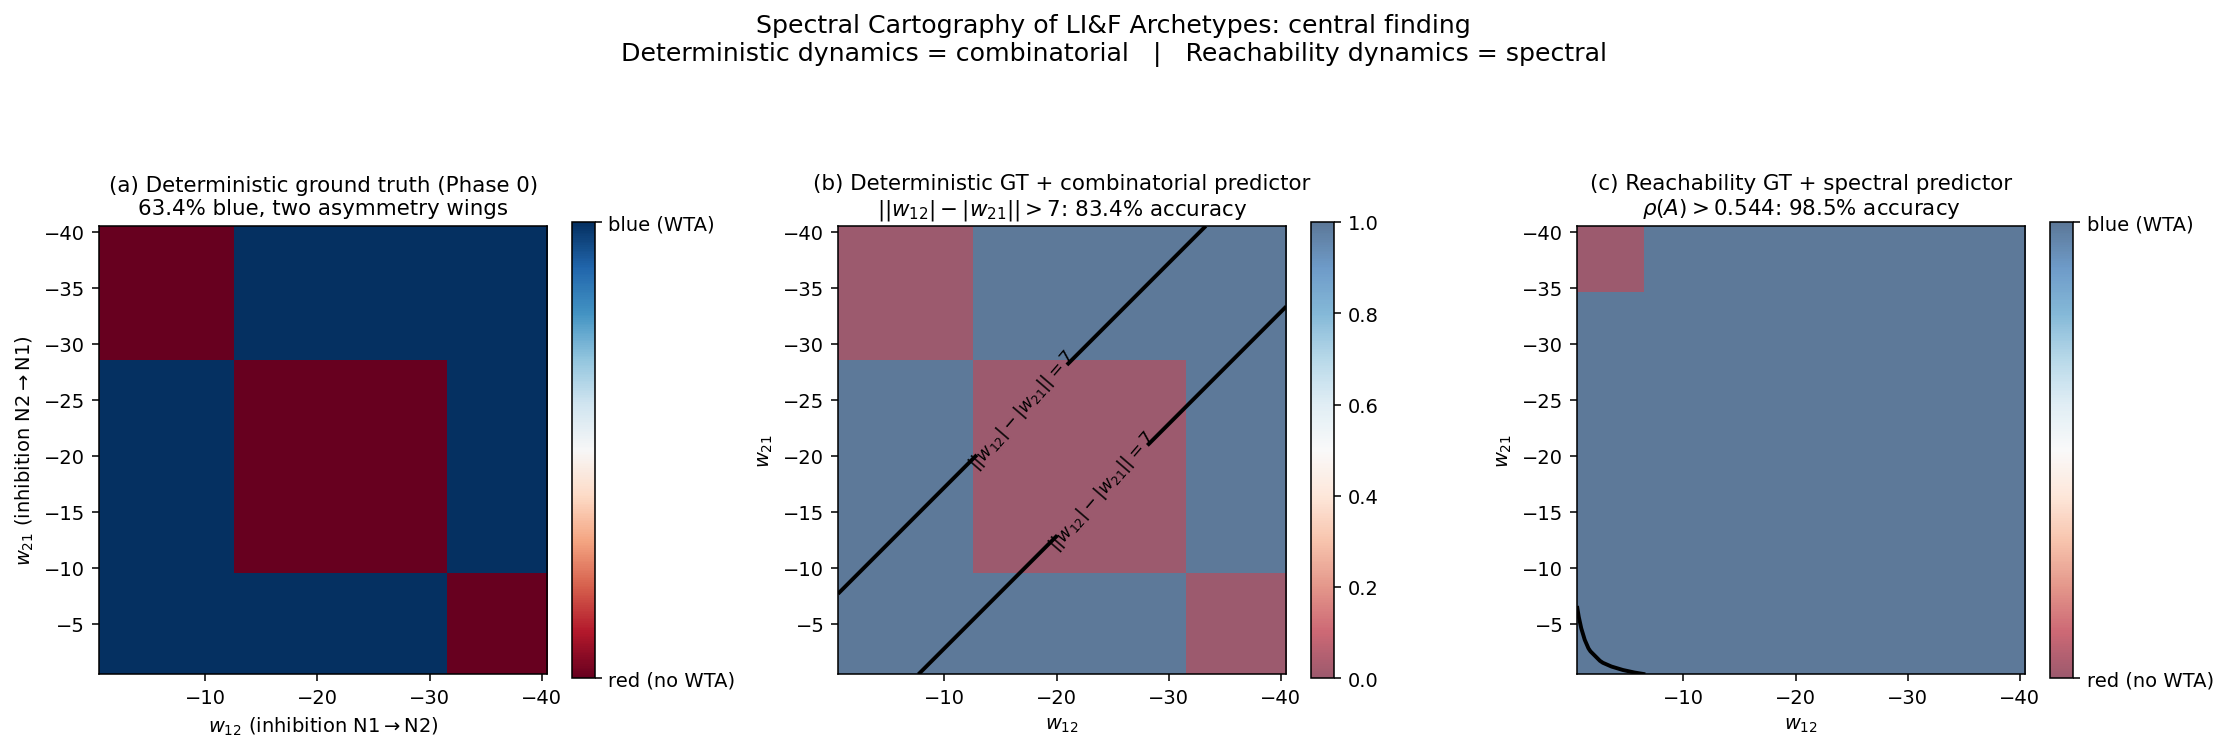
\includegraphics[width=\textwidth]{figs/triptych.png}
\caption{The two-regime split. (a) Deterministic ground truth, 63.4\% WTA. (b)
The combinatorial predictor $||w_{12}|-|w_{21}||>7$ traces the deterministic
boundary at 83.4\%; no spectral quantity reaches this. (c) Reachability ground
truth, 97.8\% WTA; the spectral-radius contour $\rho(A)=0.544$ (black) bounds
the unreachable region at 98.5\%.}
\label{fig:triptych}
\end{figure*}

This split is the paper's first and sharpest instance of a general principle.
The reset is the mechanism that \emph{chooses} the winner under deterministic
semantics, so deterministic WTA is out of spectral reach; under reachability
semantics the reset's effect is averaged over perturbations, so reachability
WTA is in reach. The split is a property of the \emph{archetype class}, not of
one topology: it transfers unchanged to the delayer-augmented variant (FCS
Figure 11), where it also reproduces FCS's ``contrary to expectation''
asymmetric winner map.

The practical consequence is a \emph{sound pre-filter}. Because $\rho(A)<0.544$
never mislabels a reachable cell, it can be placed in front of a model checker:
a flagged cell is provably not winner-take-all under the verified semantics, and
need not be checked. This composes a polynomial-cost continuous stage with the
exponential discrete one --- the multi-scale workflow of Sec.~\ref{sec:ladder}.

% ============================================================================
\section{Bifurcation structure under a population lift}\label{sec:bifurcation}
% ============================================================================

The reset blocks bifurcation theory because bifurcation theory needs a smooth
system. The population lift of rung 3 supplies one. Replacing each
contralateral neuron by a Wilson--Cowan population pair turns the
winner-take-all boundary into a \emph{bifurcation curve} that can be written
down.

Linearizing the rate equation and decomposing into symmetric and antisymmetric
modes shows the symmetric ``no-winner'' state loses stability exactly when the
\emph{loop gain} --- the product $w_{12} w_{21} g_1 g_2$ of the two weights and
the two response gains --- crosses $1$. This is a \emph{pitchfork}
bifurcation, and the loop-gain-unity condition is the classical \emph{Barkhausen
criterion} of feedback electronics. Because perturbations \emph{multiply}
around a loop, the boundary is a curve of constant product --- a hyperbola.

\par\smallskip\noindent\textbf{Finding.} In the mean-field description,
winner-take-all is an \emph{exactly solvable} bifurcation. The boundary is the
loop-gain-unity hyperbola $w_{12} w_{21} g_1 g_2 = 1$; the dominant mean-field
eigenvalue classifies cells against it at 99.96\% on a $50 \times 50$ grid, and
the symbolic pitchfork curve matches the numerical bifurcation trace to machine
precision. The whole archetype taxonomy follows: contralateral inhibition gives
a pitchfork, the negative loop a Hopf bifurcation, the positive loop a
saddle-node --- the sign of the loop's weight product selecting which.
\par\smallskip

This is the ``shape invisible to the discrete lens'' the programme set out to
find: a single eigenvalue, an analytic curve, in place of an exponential
cell-by-cell sweep. But the mean-field boundary is not the \emph{discrete}
boundary.

\par\smallskip\noindent\textbf{Negative result.} The Wilson--Cowan pitchfork is
a \emph{lower bound} on the discrete winner-take-all region, not its envelope.
Cross-validated against the LI\&F simulator, the smooth hyperbola agrees only at
the symmetric corner; the discrete bistable region is a pair of
\emph{rectangular strips} (a winner emerges once \emph{either} weight exceeds
$\approx 7$). Once either neuron fires first, its inhibition can lock the other
below threshold --- a \emph{spike-timing lock-in} that the smooth average,
having discarded the reset, has no term for.
\par\smallskip

The right reading is not ``the mean-field model is wrong'' but ``there are
\emph{two mechanisms of bistability at two scales}'': a smooth symmetry-breaking
captured by rung 3, and a discrete spike-timing lock-in that is not. They are
complementary. The continuous lens delivers the shape; the discrete lens owns
the timing.

\begin{figure*}[t]
\centering
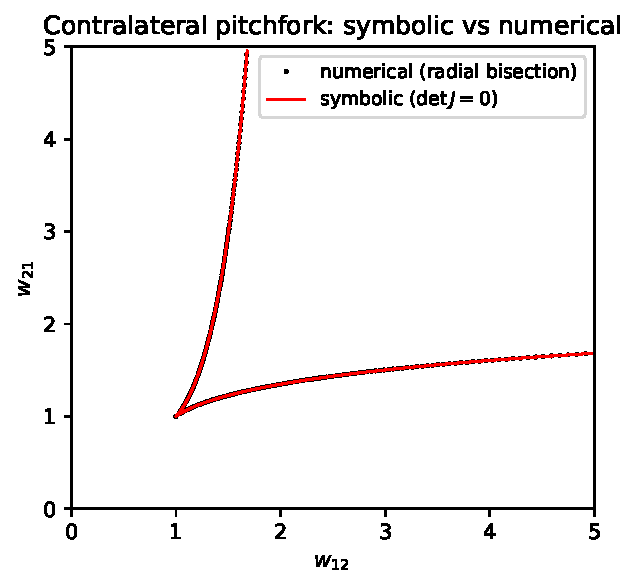
\includegraphics[width=.48\textwidth]{figs/pitchfork.pdf}\hfill
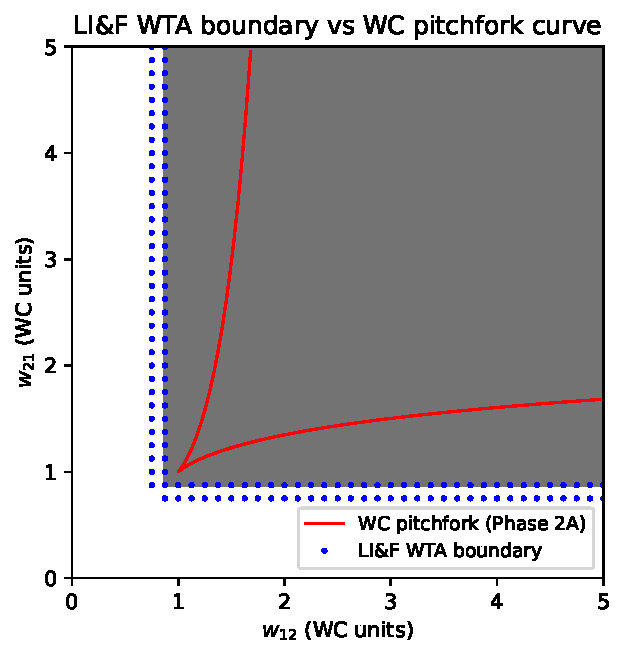
\includegraphics[width=.48\textwidth]{figs/wc_lif_overlay.pdf}
\caption{\emph{Left:} the mean-field winner-take-all region with its symbolic
pitchfork curve; a single eigenvalue classifies it at 99.96\%. \emph{Right:} the
discrete bistable region (grey) against the same pitchfork (red) --- they agree
at the symmetric corner and diverge in the arms, where spike-timing lock-in
dominates.}
\label{fig:pitchfork}
\end{figure*}

% ============================================================================
\section{Three physically-derived lenses on the discrete oracle}\label{sec:lenses}
% ============================================================================

Rung 3 still rests on a hand-tuned gain curve. Rungs 4--5 replace it with three
physically-derived objects --- the Siegert static rate, the Richardson transfer
function, the Naud--Gerstner quasi-renewal mesoscopic --- and read the discrete
FCS staircase grid through each.

\textbf{Siegert: a high-recall envelope.} Enumerating the self-consistent fixed
points of the Siegert rate equation classifies a cell as
winner-take-all-capable when a bistable pair of rates exists.

\par\smallskip\noindent\textbf{Finding.} The Siegert fixed-point map is a
high-recall \emph{envelope} of the FCS winner-take-all region: it recovers
99.6\% of the verified WTA cells. Its errors are one-sided --- it labels the
staircase blocks as WTA where the oracle does not --- because rate-equation
bistability is \emph{necessary} but not \emph{sufficient}: the staircase cells
are bistable in the rate description, yet the integer-tick dynamics never
commit. The one-sided error makes the envelope a \emph{sound pre-filter}: a cell
outside it is guaranteed non-WTA.
\par\smallskip

\textbf{Transfer function: orthogonal to the staircase.} It is tempting to read
the staircase --- where the discrete system fails to \emph{commit} in four
ticks --- as a slow-dynamics effect, and to separate it with a
transfer-function latency gate.

\par\smallskip\noindent\textbf{Negative result.} The transfer-function latency
gate is \emph{orthogonal} to the staircase: gating by the slowest-mode decay
rate changes agreement with the oracle by $-0.003$. The staircase cells are not
slow-decay cells --- they have well-separated fixed points and respectable
decay rates. Their redness is integer-tick determinism, which leaves no
signature in any linear timescale.
\par\smallskip

\textbf{Quasi-renewal: partial dissolution, and a structural floor.}
Finite-size noise can knock a fragile synchronous lock off its orbit, partially
dissolving the staircase. It does --- agreement with the oracle is best at small
population size ($0.701$ Jaccard at $N=50$, peaking near $0.717$) --- but the
improvement over the static envelope is modest, and unimodal in $N$: too much
noise also destabilises genuine WTA cells.

\par\smallskip\noindent\textbf{Finding.} No rate-equation method --- across all
of rungs 1--5 --- exceeds a Jaccard agreement of about $0.70$ with the discrete
winner-take-all oracle. This $\approx 0.70$ floor is structural. The residual
$\approx 0.30$ is the integer-tick synchronous lock, and it is the \emph{positive
content of formal verification}: a feature of the dynamics --- deterministic
spike-timing lock with phase memory --- that no rate-and-hazard theory can
express, and that only the discrete oracle resolves.
\par\smallskip

\begin{figure*}[t]
\centering
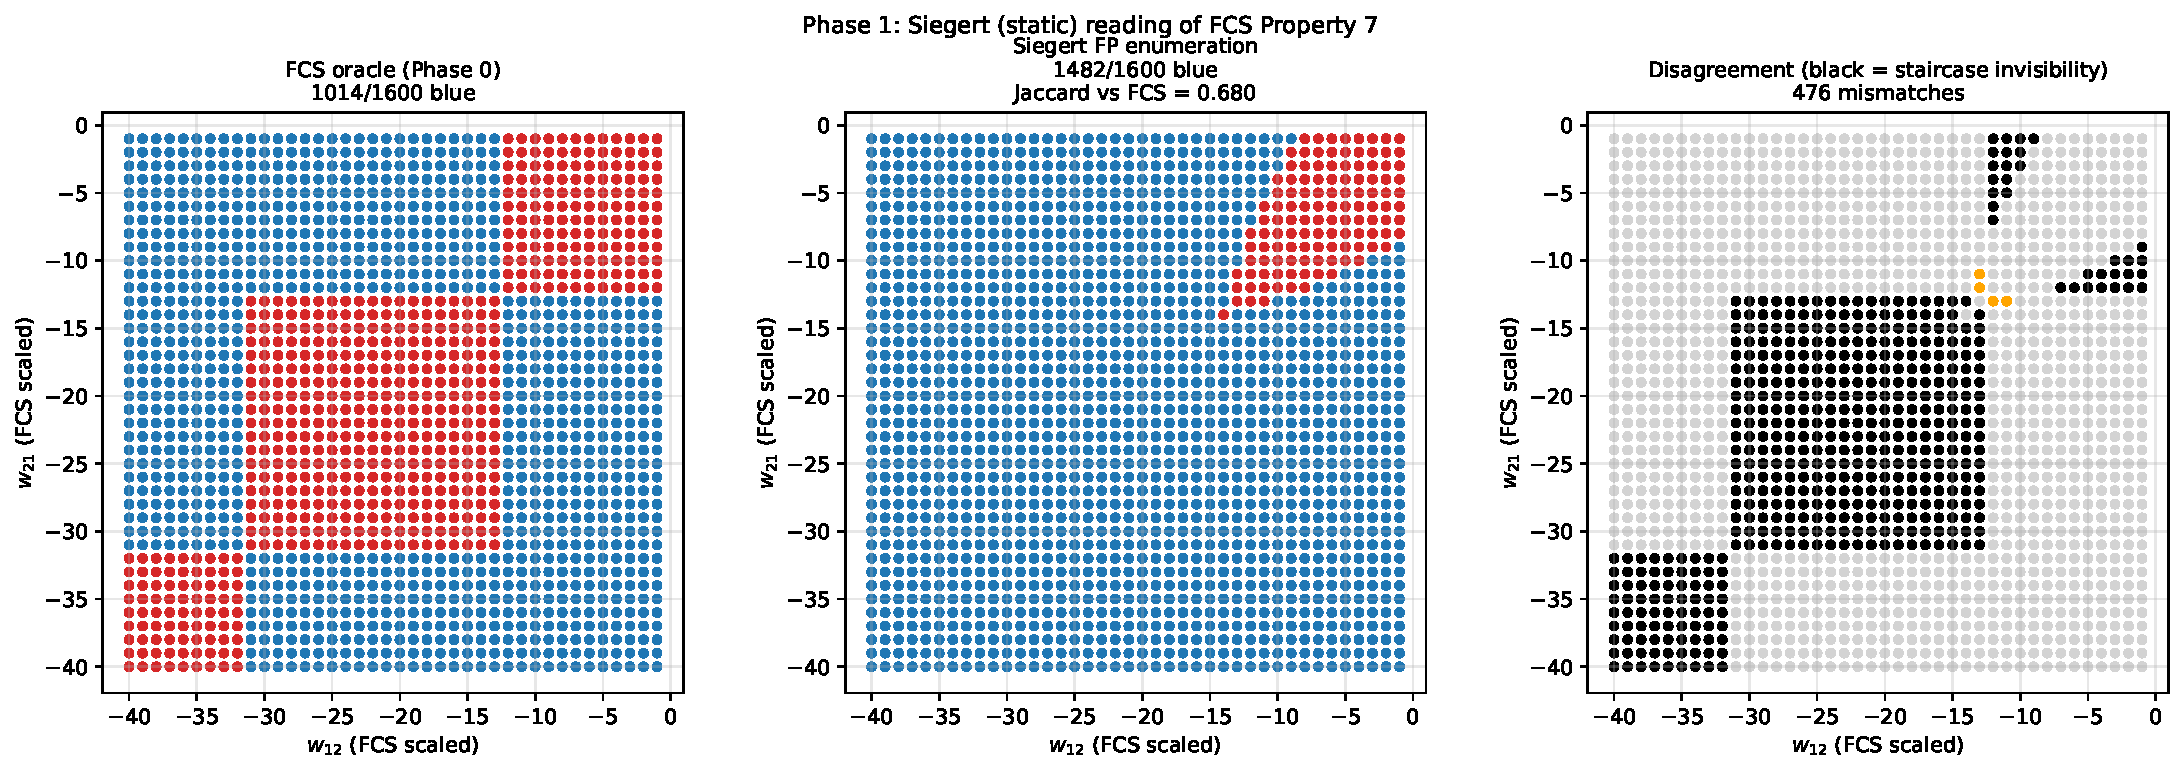
\includegraphics[width=.96\textwidth]{figs/siegert_envelope.pdf}
\caption{Rungs 4--5 on winner-take-all. Left: the discrete oracle. Centre: the
Siegert envelope. Right: the disagreement --- black cells are the diagonal
staircase, recovered as one-sided false positives. Siegert captures 99.6\% of
verified WTA cells; the staircase is the structural residual.}
\label{fig:envelope}
\end{figure*}

\textbf{The inverse staircase.} Extending the archetype from two neurons to
$N>2$ adds a \emph{second}, opposite failure.

\par\smallskip\noindent\textbf{Negative result.} The high-recall Siegert
envelope is a two-neuron luxury. For $N>2$, recall collapses with $N$ (from
$0.90$ at $N=2$ to $0.00$ at $N=10$), and at large $N$ the discrete oracle shows
clean winner-take-all \emph{below} the smooth-rate bifurcation threshold --- in
cells where the rate equations admit only the symmetric no-winner fixed point.
At $N=2$ the continuous lens \emph{over}-predicts winner-take-all (the
staircase); at $N=10$ it \emph{under}-predicts it (the \emph{inverse
staircase}). The continuous lens is wrong on both sides of the discrete
boundary.
\par\smallskip

% ============================================================================
\section{The negative loop: oscillation beyond mean field}\label{sec:oscillation}
% ============================================================================

Oscillation exposes the ladder differently, because here the mean-field theory
cannot even produce the phenomenon. For the negative loop the rate-equation
fixed point is, for \emph{every} weight choice, a \emph{stable spiral} --- the
system rings and then settles. FCS Property 5's \emph{sustained} period-$4$
oscillation is therefore not a bifurcation of the rate equations; it lies
strictly beyond mean-field reach.

The transfer function does better --- it correctly says the loop rings, and that
the ringing rate grows with the inhibition --- but its \emph{period} is wrong.

\par\smallskip\noindent\textbf{Negative result.} The transfer-function period
prediction is too long by a \emph{structural factor of about four}: across the
FCS period-$4$ region the prediction lands on the line $T_{\text{pred}} = 4
T_{\text{FCS}}$, a constant multiple. The natural fix --- recalibrate the time
constant on dynamic data --- was tested and \emph{falsified}: it widened the
gap. At the oscillation frequency the neuron's linear-response magnitude is
$\approx 0.075$, essentially flat; the oscillation lives deep in the filter's
rolled-off regime, where no single-pole model at any time constant has a
resonance to offer. The factor of four is not a calibration error --- it is an
\emph{impossibility result}: no single-pole transfer function can predict this
period.
\par\smallskip

Quasi-renewal, which carries the reset through the age distribution, succeeds
where the transfer function structurally cannot.

\par\smallskip\noindent\textbf{Finding.} Quasi-renewal recovers the oscillation
period. Using the same calibration the transfer function used, it predicts
$4.05$ ticks at the default cell --- essentially exact --- because its
age-distribution stepper represents spike-and-reset explicitly, and ``reset'' is
precisely what a single-pole filter cannot express. The sustained oscillation
itself is finite-size: its amplitude decays as $N$ grows, confirming a
noise-driven cycle around a fixed point that, deterministically, only spirals
inward.
\par\smallskip

What no rate method delivers is the \emph{binary} \texttt{1100} waveform: a rate
is smooth, so even an exact-period prediction matches the binary template only
weakly. The period scales as $2(n+1)$ in the number of delayer stages, and
quasi-renewal tracks that scaling; the transfer function stays structurally
wrong. The ladder's verdict on oscillation generalises.

\begin{figure*}[t]
\centering
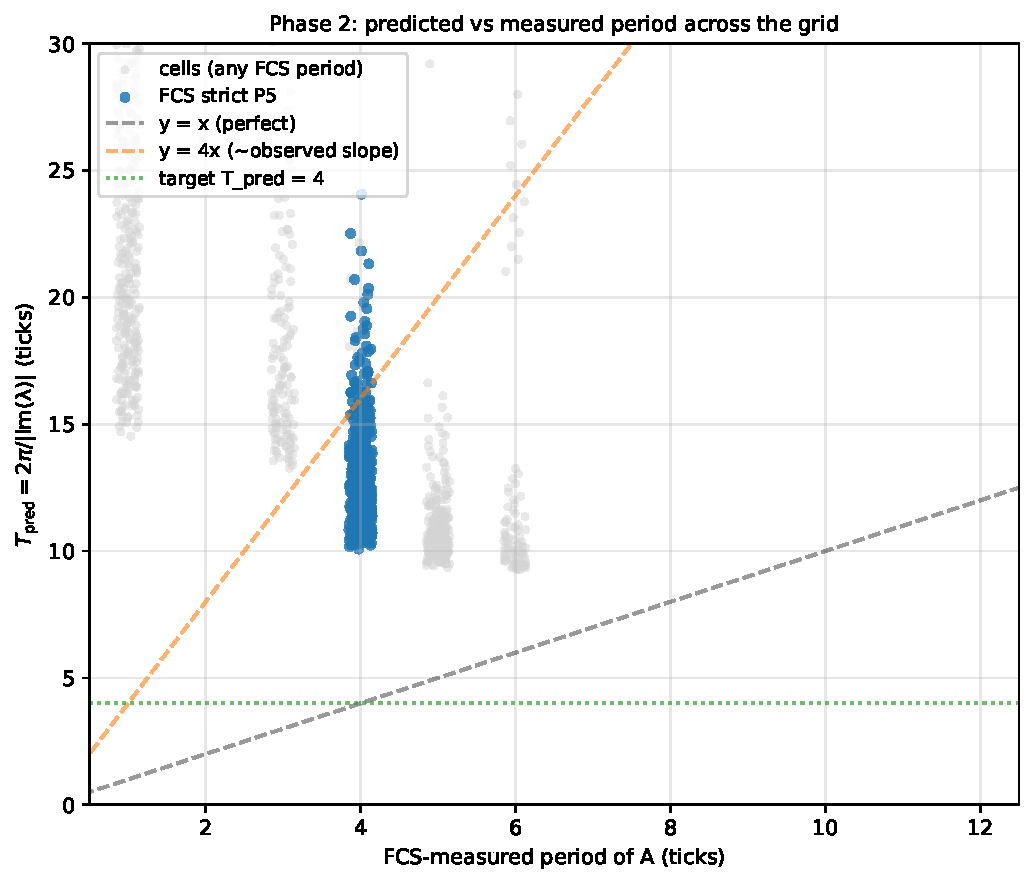
\includegraphics[width=.48\textwidth]{figs/negloop_Hw_period.pdf}\hfill
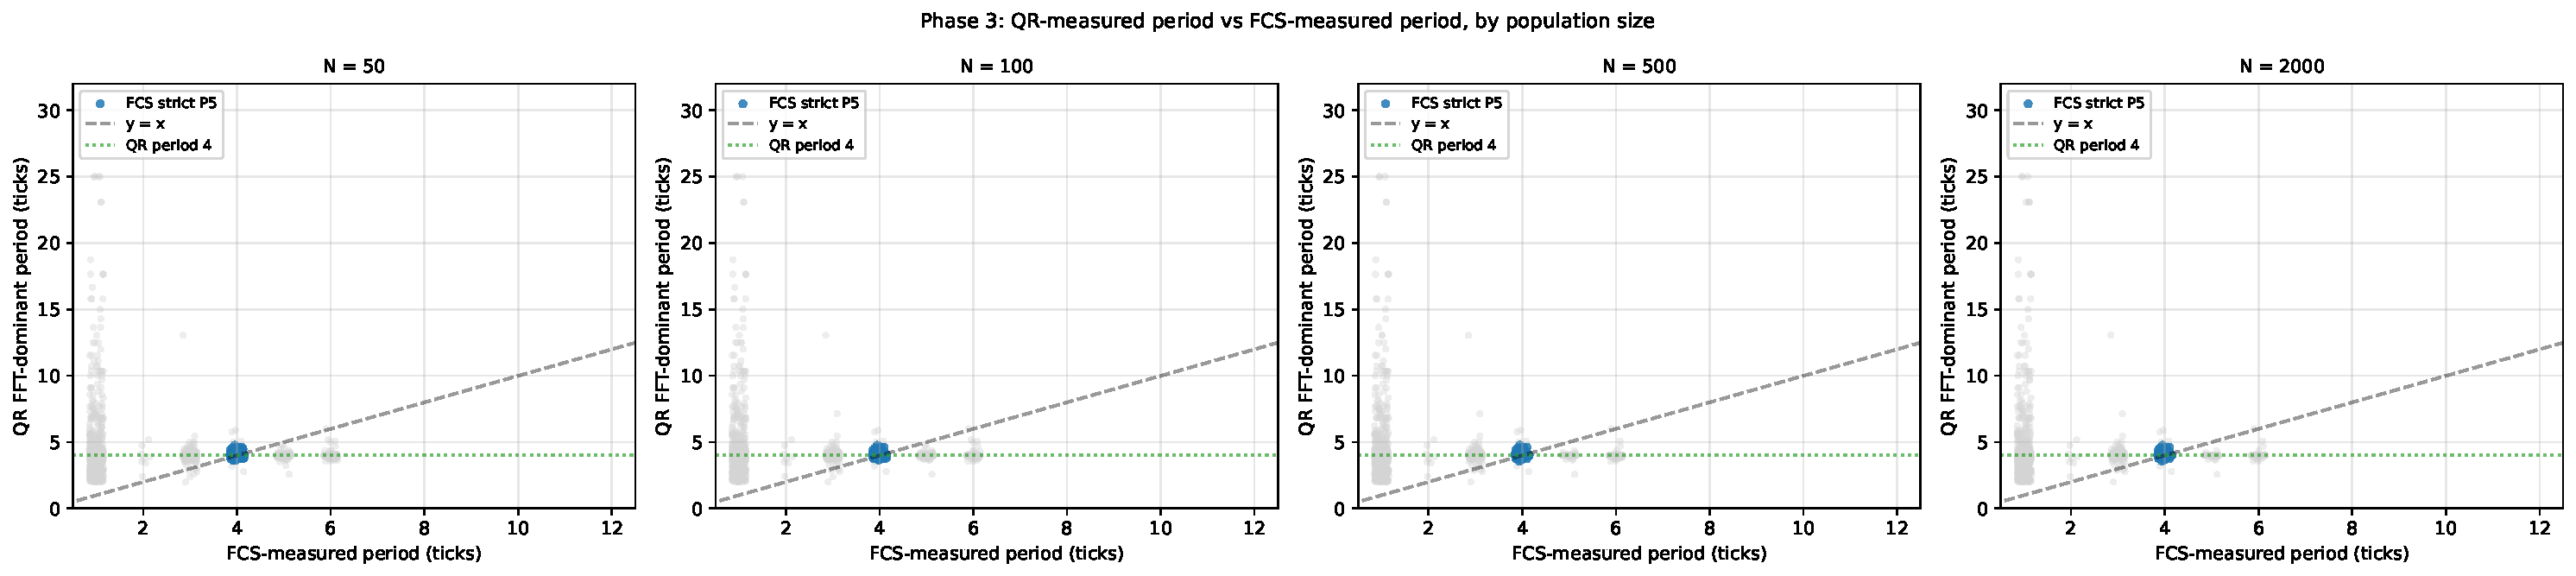
\includegraphics[width=.48\textwidth]{figs/negloop_qr_period.pdf}
\caption{Oscillation period. \emph{Left:} the transfer-function prediction lands
on $T_{\text{pred}}=4 T_{\text{FCS}}$ (orange) --- a structural overshoot.
\emph{Right:} quasi-renewal lands on the diagonal $T=T_{\text{FCS}}$ --- the
correct integer-tick period.}
\label{fig:period}
\end{figure*}

% ============================================================================
\section{The methodology ladder and a multi-scale workflow}\label{sec:ladder}
% ============================================================================

The results above climb the ladder of Table~\ref{tbl:ladder} twice, once per
phenomenon, and the pattern is the same each time. Rungs 1--5 pass on the
questions of \emph{shape and existence} --- is there a winner, where is the
boundary, can the target be reached, does the loop ring --- and fail on the
questions of \emph{exact integer schedule} --- which staircase cell, which
period, which waveform. Only rung 6 passes everywhere, at exponential cost. The
boundary between the two is a single mechanism.

\par\smallskip\noindent\textbf{The diagnostic principle.} The spike-reset rule
is the essential nonlinearity that continuous analysis erases. Whether it
appears in the formal property being verified is a decidable, a-priori test for
whether continuous methods are sound for it. Properties about the existence and
stability of attractors --- reachability, bifurcation, oscillatory-versus-not
classification --- do not depend on the exact reset schedule, and rungs 1--5
reach them. Properties about the exact integer schedule of spikes ---
deterministic trajectories, integer periods, binary waveforms, deterministic
lock-in --- are the reset schedule, and only rung 6 reaches them.
\par\smallskip

The principle is not asserted; it is \emph{confirmed}. It is confirmed
positively by the spectral reachability certificate (Sec.~\ref{sec:wta}), the
exact bifurcation curves (Sec.~\ref{sec:bifurcation}), and the Siegert envelope
(Sec.~\ref{sec:lenses}). It is confirmed negatively by four failed hypotheses,
each of which tried to extract a fact about the integer reset schedule from a
continuous description and failed exactly where the principle predicts: the
eigenvalue gap on deterministic winner-take-all; the latency gate on the
staircase; the transfer-function period (an impossibility result,
Sec.~\ref{sec:oscillation}); the Wilson--Cowan pitchfork as the discrete
boundary (Sec.~\ref{sec:bifurcation}). Negative results that fall where a
principle predicts are evidence \emph{for} the principle; reported together, the
four failures \emph{measure} the boundary of continuous analysis rather than
merely encountering it.

The principle has an engineering corollary: a \emph{multi-scale verification
workflow}. Run the cheap continuous rungs first as a \emph{pre-filter and
hypothesis generator}; the sound certificate $\rho(A)<0.544$ provably eliminates
cells from the model checker's workload, and the bifurcation curves and Siegert
envelope locate the regions where behaviour changes. Reserve the exponential
discrete model checker for exactly the cells the diagnostic principle marks as
reset-dependent --- the staircase, the exact period, the waveform. The
continuous lens does not replace formal verification; it \emph{delimits} it, and
the delimitation is decidable before either tool is run.

% ============================================================================
\section{Related work}\label{sec:related}
% ============================================================================

Formal verification of SNN archetypes was established by De Maria et al.
\cite{DeMaria2020,naco20} (Lustre/Kind2 model checking, the FCS programme) and
extended to probabilistic neurons and PRISM by the CogSpike line
\cite{cogspike_wd,yao2025probabilistic}. That body of work is \emph{discrete
throughout}. The continuous neuron-modelling tradition this paper draws on is
equally established but separate: Wilson--Cowan population rate equations
\cite{WilsonCowan1972} and lateral-inhibition neural fields \cite{Amari1977};
the Siegert first-passage firing rate \cite{Siegert1951} and its use in network
theory \cite{Brunel2000,BrunelHakim1999}; the linear-response transfer function
of integrate-and-fire neurons \cite{Richardson2007}; and finite-size mesoscopic
population equations \cite{NaudGerstner2012,Schwalger2017}. Bifurcation theory
is standard \cite{Strogatz2014,Kuznetsov2004}.

The contribution of this paper is at the \emph{seam} between these two
traditions. Prior work either verifies SNN properties discretely or models SNN
dynamics continuously; we hold the continuous models against a bit-exact
discrete verification oracle, on the same archetypes, and characterise precisely
which formal properties survive the continuous reduction. The diagnostic
principle --- the spike-reset rule as a decidable scope boundary --- and the
two-regime characterisation of winner-take-all are, to our knowledge, new.

% ============================================================================
\section{Conclusion and outlook}\label{sec:conclusion}
% ============================================================================

A continuous, differential-equation lens does reveal structure in LI\&F
spiking-network archetypes that exhaustive discrete verification does not: a
single eigenvalue predicts the winner-take-all boundary at 99.96\% in
mean-field; the winner-take-all and oscillation-onset boundaries are exact
closed-form curves; the Siegert formula yields a 99.6\%-recall, soundly
one-sided envelope of the verified region. But the lens has a sharp and
\emph{identifiable} limit. The spike-reset rule is the one nonlinearity every
continuous method erases, and whether it is load-bearing for a property is a
decidable test for whether continuous analysis is sound. Properties of shape and
existence are in scope; properties of the exact integer spike schedule --- the
staircase, the period, the binary waveform --- are not, and the residual
disagreement between every continuous method and the discrete oracle (a Jaccard
floor of $\approx 0.70$, a structural factor-of-four period gap) is a
\emph{measurement} of how much of a verified property is irreducibly discrete.

The continuous and the discrete lenses are complementary, and the diagnostic
principle is the contract between them: it says, before either is run, which
questions the cheap continuous lens answers and which must go to the exponential
model checker. The most direct engineering outcome is the sound spectral
pre-filter; developing it into a tool composed against a concrete Lustre
encoding is the natural next step. The most promising theoretical direction is a
\emph{hybrid-system} spectral theory --- saltation matrices or Floquet theory of
periodic-reset systems \cite{KhalilNonlinear} --- whose spectrum would carry the
reset frequency explicitly, and which could, in principle, build the rung
between mesoscopics and the discrete oracle that finally reaches the integer
period.

\bibliographystyle{IEEEtran}
\bibliography{refs}

\end{document}
